\section{Gebruikers Beschrijving}

\subsection{Belanghebbenden}
In deze sectie van het SRD worden de belanghebbende van de opdracht geïdentificeerd. Er zal ook worden beschreven wat de behoeften zijn van de belanghebbenden, die uiteindelijk zullen worden overwogen in het ontwerpproces.

\textbf{Belanghebbenden:}

\begin{itemize}
	\item \textbf{Customer Service (Hoofdgebruiker van de testkast)}
	\begin{itemize}
		\item De customer serviceafdeling zal de testkast gaan gebruiken om teruggestuurde spindels te testen en te analyseren. De behoeften van deze afdeling zullen zijn:
		\begin{enumerate}
			\item Een gebruiksvriendelijke interface om verschillende spindels te testen op de testkast.
			
			\item De testresultaten moeten betrouwbaar zijn en reproduceerbaar.
			
			\item Log bestanden en testrapporten om analyses uit te voeren.
			
			\item Test criteria waar de motoren aan moeten voldoen zodat ze als goed of slecht kunnen worden bestempeld.
			
			\item Meerdere soorten motoren moeten werken op de testkast.
			
			\item Documentatie om de kast te bedienen.
		\end{enumerate}
	\end{itemize}
	
	\item \textbf{Operators (Dagelijkse gebruikers van de testkast)}
	\begin{itemize}
		\item De operators van de testkast zijn de mensen die de kast daadwerkelijk gaan gebruiken. Hun behoeften kunnen zijn:
		\begin{enumerate}
			\item Een gemakkelijke manier om de testparameters voor een specifieke spindel te selecteren.
			
			\item Een veilig systeem wat de risico’s minimaliseert tijdens het testen van de spindels.
			
			\item Een testproces wat niet te veel tijd kost.
			
			\item Duidelijke feedback van de testkast als eventuele problemen zich voor doen. (Foutmeldingen of waarschuwingen)
			
			\item Eventueel vertaalde tekst op het scherm in andere talen.
		\end{enumerate}
	\end{itemize}
	
	\item \textbf{Onderhoudsdienst}
	\begin{itemize}
		\item De onderhoudsdienst is verantwoordelijk voor het onderhoud van de testkast en eventuele uitbreiding van de kast. De behoeften van deze groep is:
		\begin{enumerate}
			\item Goede documentatie van de code.
			
			\item Inzicht in de parameters en instellingen van de testkast.
			
			\item Goed documentatie van de hardware.
		\end{enumerate}
	\end{itemize}
	
	\item \textbf{R\&D Engineering Team}
	\begin{itemize}
		\item Wanneer Voortman besluit nieuwe machines te ontwikkelen met mogelijk nieuwe type spindels kan de testkast ook nuttig zijn voor de R\&D. Zij zouden de volgende dingen willen:
		\begin{enumerate}
			\item Makkelijk nieuwe testscenario’s kunnen instellen voor de nieuwe motoren.
			
			\item Overzicht over de prestaties van de spindel.
		\end{enumerate}
	\end{itemize}
	
	\item \textbf{Klanten van Voortman}
	\begin{itemize}
		\item Klanten die de gereviseerde motor uiteindelijk kopen kunnen ook baat hebben bij de testkast zij zouden de volgende dingen willen hebben:
		\begin{enumerate}
			\item Een testrapport waarin te zien is dat de gekochte gereviseerde spindel correct werkt naar behoren.
		\end{enumerate}
	\end{itemize}
\end{itemize}

\newpage

\subsection{Gebruikersscenario(s)}

In deze sectie worden alle verschillende gebruikersscenario’s geschetst om de interactie die de gebruiker heeft met het systeem te visualiseren. De volgende stappen moeten doorlopen worden om de spindel juist aan te sluiten en te testen op de testkast.

\begin{figure}[H]
	\centering
	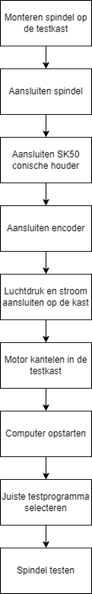
\includegraphics[width=0.18\linewidth]{Gebruikersscenario}
	\label{fig:Gebruikersscenario}
	\caption{Gebruikersscenario spindel bedienen}
\end{figure}

\newpage

\begin{itemize}
	\item \textbf{Monteren spindel op de testkast} houdt in dat de spindel met tenminste twee bouten wordt vastgedraaid op de testkast zodat deze niet meer kan bewegen.
	
	\item \textbf{Aansluiten spindel} betekent dat de drive wordt aangesloten op de spindel.
	
	\item \textbf{Aansluiten SK50 conische houder} betekent dat de luchtcilinders worden aangesloten op de testkast en dat de sensor die checkt of de houder goed gesloten is aangesloten wordt.
	
	\item \textbf{Aansluiten encoder} houdt in dat de encoder wordt aangesloten op de motordrive.
	
	\item \textbf{Luchtdruk en stroom aansluiten op de testkast} houdt in dat de testkast aangesloten wordt op het lichtnet en op de luchtdruk.
	
	\item \textbf{Motor kantelen in de testkast} houdt in dat de spindel wordt gekanteld doormiddel van een Linak actuator binnen in de testkast dit zorgt ervoor dat het draaiende gedeelte van de spindel niet of moeilijker bereikbaar wordt voor de gebruiker dit waarborgt de veiligheid van de gebruiker.
	
	\item \textbf{Computer opstarten} nu alles gereed is kan de computer opgestart worden het testprogramma zou automatisch moeten verschijnen.
	
	\item \textbf{Juist programma kiezen} wanneer de computer is opgestart kan er een testprogramma worden gekozen de juiste parameters worden dan in de drive geladen en de spindel is klaar om getest te worden.
	
	\item \textbf{Spindel testen} de spindel kan nu getest worden.
\end{itemize}

\newpage

\subsection{Voorbeeld eis}

In deze sectie is een kort voorbeeld gemaakt over hoe de eisen in elkaar zitten. Dit is te zien in \ref{tab:Uniek ID}.

% Makkelijk command om eisen in te voegen
\newcommand{\eistabel}[6]{
	\begin{table}[H]
		\centering
		\caption{#1 #2}
		\label{tab:#1}
		\begin{tabular}{|p{0.15\linewidth}|p{0.5\linewidth}|p{0.2\linewidth}|}
			\hline
			\textbf{#1} & \textbf{#2} & \textbf{#3} \\
			\hline
			\textbf{Stelling} & \multicolumn{2}{p{0.7\linewidth}|}{#4}\\ 
			\hline
			\textbf{Meetmethode} & \multicolumn{2}{p{0.7\linewidth}|}{#5} \\ 
			\hline
			\textbf{Opmerking} & \multicolumn{2}{p{0.7\linewidth}|}{#6} \\ 
			\hline
		\end{tabular}
	\end{table}
}

\eistabel{Uniek ID}{Titel}{Prioriteit}{Eis van de stelling}{Meetmethode}{Eventuele opmerkingen}

De bovenste rij van de tabel geeft de volgende dingen weer:

\begin{itemize}
	\item \textbf{Uniek ID}
	\begin{itemize}
		\item Elke eis heeft zijn eigen unieke ID zodat hier later naar verwezen kan worden.
	\end{itemize}
	
	\item \textbf{Titel}
	\begin{itemize}
		\item Elke eis heeft zijn eigen titel die kort de eis beschrijft.
	\end{itemize}
	
	\item \textbf{Prioriteit}
	\begin{itemize}
		\item Niet elke eis is urgent en daarom heeft elke eis zijn eigen prioriteit. Er zijn vier prioriteiten: URGENT, HOOG, GEMIDDELD en LAAG.
	\end{itemize}
\end{itemize}

De rest van de tabel omvat het volgende:

\begin{itemize}
	\item \textbf{Stelling}
	\begin{itemize}
		\item Een duidelijke en beknopte beschrijving van de eis.
	\end{itemize}
	
	\item \textbf{Meetmethode}
	\begin{itemize}
		\item Een methode hoe de eis gevalideerd gaat worden in de testfase van het project.
	\end{itemize}
	
	\item \textbf{Opmerking}
	\begin{itemize}
		\item Om onduidelijkheden te verhelpen kan er nog een aanvullende opmerking worden toegevoegd in deze rij.
	\end{itemize}
\end{itemize}

\subsection{Functionele eisen}

\eistabel{FR-001}{Geautomatiseerd testen}{URGENT}{De testkast moet in staat zijn om geautomatiseerd te kunnen testen. Dit houdt in dat er testen gemaakt moeten kunnen worden die vervolgens uitgevoerd kunnen worden op de testkast.}{De eis is behaald wanneer een operator, die los staat van dit project, op de testkast een test kan maken met het instructieboekje en deze ook kan afspelen op de testkast. Deze testkast moet deze test dan automatisch afspelen.}{De operator moet tenminste de keuze hebben uit welk toerental, hoe snel de spindel deze moet bereiken en voor hoelang de spindel moet draaien in dit toerental.}

\eistabel{FR-002}{Testrapport}{GEMIDDELD}{De testkast moet in staat zijn om na afloop van de test een rapport te maken waarin de resultaten van de test staan.}{De eis is behaald wanneer het programma op de testkast een testrapport maakt na afloop van de test. De door de operator gekozen parameters moeten tijdens de test gemonitord worden en weergegeven worden in het rapport. Ook de hoeveelheid samples per seconde moet door de operator gekozen kunnen worden.}{}

\eistabel{FR-003}{Spindel validatie}{LAAG}{Na afloop van de test moet de testkast doormiddel van een statistische analyse van de opgenomen parameters aan kunnen geven of dit binnen de toegestane toleranties en specificaties valt, en of de spindel als ‘goed’ of ‘afgekeurd’ geclassificeerd moet worden.}{De eis is behaald wanneer de testkast spindels kan keuren op basis van tenminste het stroomverbruik deze mag niet significant afwijken van nieuwe spindels met een betrouwbaarheidsinterval van 95\%. De controlegroep moet hiervoor normaal verdeeld zijn met ideaal >30 observaties van nieuwe correct werkende spindels op verschillende toerentallen.}{}

\eistabel{FR-004}{Real time grafieken}{HOOG}{Tijdens de test moeten er op het scherm grafieken komen met real-time data van de spindel. Welke data er op het scherm moet komen moet kunnen worden gekozen door de gebruiker.}{De eis is behaald wanneer de gebruiker een willekeurige parameter kan kiezen en deze kan monitoren op de GUI tijdens de test. Ook de hoeveelheid samples per seconde moet gekozen kunnen worden door de gebruiker.}{}

\eistabel{FR-005}{Op afstand testen}{GEMIDDELD}{Wanneer de testkast bezig is moet de gebruiker op afstand de testgegevens kunnen bekijken via bijvoorbeeld het \gls{MQTT}-protocol op grafana.}{De eis is behaald wanneer de gebruiker tenminste het stroomverbruik en hoelang het testen nog duurt kan monitoren vanaf een andere laptop die niet is aangesloten op de testkast.}{}

\eistabel{FR-006}{Automatisch parameters inladen}{URGENT}{De testkast moet geautomatiseerd andere parameters in kunnen laden van andere motoren.}{De eis is behaald op het moment dat er een andere motor wordt aangesloten dat de gebruiker slechts door de motor te selecteren in de GUI de parameters kan inladen in de drive die passen bij die motor.}{}

\eistabel{FR-007}{Handmatig testen}{URGENT}{De gebruiker moet de spindels handmatig kunnen aansturen met de GUI op de testkast. }{Deze eis is behaald wanneer de gebruiker handmatig de motor kan aansturen met de GUI op de testkast.}{Het aansturen kan bijvoorbeeld met een slider.}

\eistabel{FR-008}{TwinSAFE geconfigureerd}{GEMIDDELD}{De veiligheidskritieke onderdelen in de testkast zoals de deurschakelaars maar ook de motordrive moeten worden geconfigureerd in een TwinSAFE project zodat de veiligheid van de gebruiker te allen tijde kan worden gewaarborgd.}{Deze eis is behaald wanneer de motor automatisch en gecontroleerd wordt afgeremd met een TwinSAFE project zodra één van de volgende veiligheidsvoorwaarden worden geactiveerd:
\begin{itemize}
	\item Deurbeveiliging: op het moment dat er een deur op de testkast geopend wordt.
	\item Noodstop: wanneer de noodstop wordt ingedrukt.
	\item Wanneer veiligheidslimieten worden overschreden: Bijvoorbeeld een te hoge stroomafwijking.
\end{itemize} De motor moet zo snel mogelijk afremmen. Omdat dit sterk afhankelijk is van welk type motor en welke massatraagheid de spindel heeft en mogelijk nog de tool die hierin zit kan hier geen vaste waarde aan gehangen worden.}{Momenteel is deze veiligheid al wel ingebouwd in de testkast echter is dit niet gedaan met TwinSAFE maar gewoon geprogrammeerd in een \gls{TwinCAT} \gls{PLC} project. }

\eistabel{FR-009}{Servo Motoren}{URGENT}{Tenminste de volgende motoren moeten kunnen worden aangestuurd door de AX5140 motordrive:
\begin{itemize}
	\item MAD100D-0250-SA-C0-AK0-35-N3 (V623) Async servo motor
	\item MAD130C-0150-SA-S2-AP0-05-N1 (V633, V310 nieuw) Async servo motor
	\item HQL100X (V310 oud) Async servo motor
	\item MSK101D-0450-NN-M1-AP0-NNNN (V505-250T, V320, V330C, V320C en V600) Sync servo motor
	\item MS2N10-D0BNN-AMVK0-NNNNN-NN (V630 nieuw)  Sync servo motor
	\end{itemize}}{Deze eis is behaald wanneer bovenstaande motoren aangestuurd kunnen worden vanaf de drive de motoren moeten hierbij draaien.}{Het aansturen kan bijvoorbeeld met een slider.}

\eistabel{FR-010}{FFT-analyse}{LAAG}{De Testkast moet een Fast Fourier Analysis (\gls{FFT}) kunnen uitvoeren op de gemeten trilling gegevens om frequentiespectra te genereren.}{De eis is behaald wanneer de testkast de spindel die getest wordt kan vergelijken met een aantal juist werkende spindels op basis van de trillingen van de motor en ook kan aangeven waar de verschillen zitten om zo mogelijke problemen aan te kunnen duiden.
	
	\vspace{0.5cm}
Meet eerst de trillingen van de motor bij de volgende snelheden:
	
\begin{itemize}
	\item \textit{20\% van de maximumsnelheid}
	\item \textit{50\% van de maximumsnelheid}
	\item \textit{80\% van de maximumsnelheid}
\end{itemize}

Doe vervolgens de transformatie voor elke dataset. De formule voor de \gls{DFT} (Discrete Fourier Transform) is (voor grote datasets is het Cooley–Tukey \gls{FFT} algorithm sneller) \cite{web:FFT,web:Radix-2FFT}
}{}
